\chapter{Conoscenze preliminari}
\label{ch:Conoscenze Preliminari}
\section{Generalità sulle reti neurali}
Le reti neurali, spesso chiamate anche reti neurali artificiali o simulate, sono algoritmi con nomi e strutture 
ispirate al cervello umano ed hanno lo scopo di ricreare il modo in cui i neuroni umani comunicano.
Le reti artificiali sono, nella maggior parte dei casi, sistemi adattivo, ovvero possono cambiare
la propria struttura in base alle informazioni che circolano all'interno della rete.
Una rete neurale non è altro che una funzione matematica. Una rete neurale solitamente è definita 
da una serie di neuroni (vedi sezione \ref{Neuroni nelle reti neurali}) connessi tra di loro.
% strutturazione delle reti neurali
Usualmente le reti artificiali sono composte da più livelli: un livello relativo alla gestione dell'input,
uno o più livelli nascosti ed un livello per la gestione degli output.
Ogni livello è composto da nodi o neuroni artificiali.
La connessione tra ognuno di questi nodi avviene mediante l'uso di soglie e pesi. Se, ad esempio, 
l'output generato da un nodo è al di sopra di una soglia specificata, il nodo viene attivato in modo 
da inviare dati al livello successivo della rete, altrimenti non vengono inviati dati.
\\\\
Ogni neurone è composto da dati di input, pesi, una soglia (detta anche bias) e dai dati restituiti in output.
una volta che le dimensioni dei dati in ingresso vengono determinati, si assegnano anche i pesi.
I pesi sono fondamentali, poiché aiutano a determinare l'importanza di ogni variabile in ingresso 
al neurone: pesi più grandi indicano che la varabile ha maggior importanza nella determinazione dell'output,
pesi minori indicano che la variabile è meno importante per la determinazione dell'output.
$\\\\$
Altro valore di rilievo è quello relativo alla soglia, poiché se il valore determinato come output supera la soglia, 
il nodo viene attivato. In tal modo vengono passati i dati al neurone successivo.
Così l'output di un nodo diventa l'input del successivo.
\\\\
All'inizializzazione della rete, i pesi vengono scelti in maniera casuale, portando la rete 
ad avere scarsi risultati. Allenare una rete significa passare da una rete poco performante ad 
una con un accuratezza elevata. Ciò è reso possibile dal fatto che possiamo modificare la funzione 
che gestisce la rete, effettuando degli accorgimenti sui pesi.
\\\\
Essendo la rete neurale una funzione, quando alleniamo la rete per avere prestazioni migliori,
ciò che facciamo è minimizzare la funzione di perdita (loss function).Esistono vari  algoritmi per ottimizzare funzioni, questi possono essere basati sul 
gradiente o meno.
\begin{figure}[h]
    \centering
    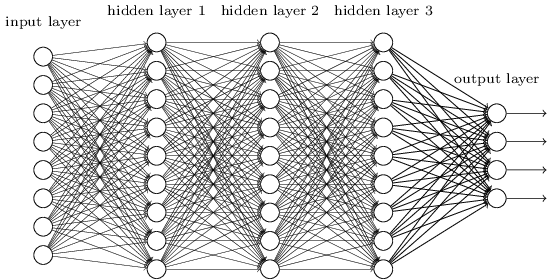
\includegraphics[width=10cm]{./neural_net.png}
    \label{neural network}
    \caption{Esempio di architettura di rete neurale}
\end{figure}
$\\\\$
In virtù del fatto che l'obiettivo è trovare il minimo della funzione, vengono effettuati tentetivi
ad ogni iterazione dell'allenamento. Un parametro fondamentale in questo processo è il \emph{learning rate}.
Tale parametro indica la grandezza del salto che viene effettuato ad ogni iterazione per avvicinarsi al 
minimo della funzione. Per tale motivo se tale valore è troppo elevato, saranno effettuati salti 
troppo grandi con il rischio di superare il minimo e conseguente divergenza dell'algoritmo.
Se, al contrario si usa un learning rate troppo piccolo i tempi per trovare il minimo potrebbero aumentare 
ed il minimo a cui si converge potrebbe essere un minimo locale.

\subsection{Struttura di un neurone artificiale}
\label{Neuroni nelle reti neurali}
Un neurone non è altro che una funzione matematica. Tale funzione ha un input, di dimensione 
determinata, e restituisce un output. Sono, inoltre, presenti 
dei coefficienti moltiplicativi fondamentali per determinare l'output chiamati pesi.
I pesi diversificano i neuroni e vengono determinati durante l'allenamento della rete, ovvero la 
fase in cui si regolano la rete.
\begin{figure}[h]
    \centering
    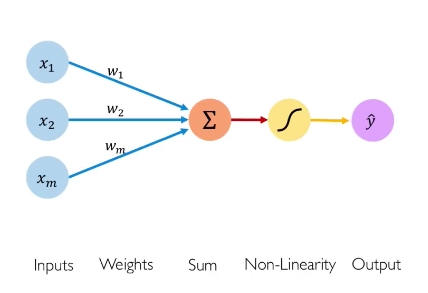
\includegraphics[width=8cm]{./neuron.png}
    \label{neuron}
    \caption{Esempio di neurone}
\end{figure}
$\\\\$
La funzione che descrive un neurone può essere divisa in due parti: combinazione lineare di 
input e pesi preceduta da una funzione non lineare. La funzione non lineare più usata è ReLU (Rectified 
Linear Unit). Tale funzione risulta essere pari a zero se $x$ è minore di zero e restituisce $x$ se tale valore 
è maggiore di zero. Oltre a ReLU esistono altre funzioni, tra cui: Sigmoid, Softmax, entrambe usata
anche nel progetto di tesi, SELU e GELU. 
Di seguito viene riportata l'espressione matematica descrivente la funzione ReLU.
\begin{equation*}
    ReLU(x)=max(x,0)
\end{equation*}
$\\\\$
Infine è utile ricordare che il valore restituito dal neurone è indicato col termine attivazione, 
poiché determina se il neurone verrà attivato, passando i dati al neurone successivo nella catena, o meno.
\subsection{Tipologie di Layer}
\label{tipologie}
Esistono vari tipi di layer usati nella creazione delle reti neurali. I tipi più comuni di layer sono quattro:
Fully connected, Convolutional, Deconvutional e Recurrent.
\begin{figure}[h]
    \centering
    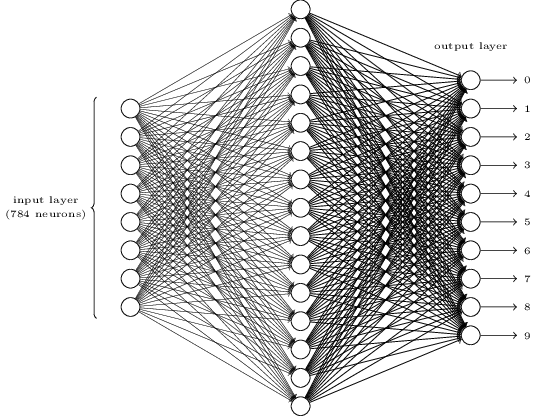
\includegraphics[width=6cm]{./dense.png}
    \label{dense}
    \caption{Esempio di dense layer}
\end{figure}
$\\$
Nel caso considerato si è deciso di usare, in particolare, layer fully connected e convolutional.
I layer fully connected sono caratterizzati dalla presenza di connessioni tra i neuroni di un layer e
i tutti i neuroni del layer successivo. Tale tipologia di layer si trova in varie reti neurali, tra cui le 
reti convoluzionali. Spesso tali layer sono chiamati anche Dense layer.
I layer convoluzionali sono i layer principali all'interno delle reti convoluzionali, a cui danno il nome.
Sono spesso usati per ricavare caratteristiche nelle immagini grazie all'uso di filtri per analizzare l'immagine stessa
prendendo pochi pixel alla volta e restituendo in output una mappa delle caratteristiche.
\begin{figure}[h]
    \centering
    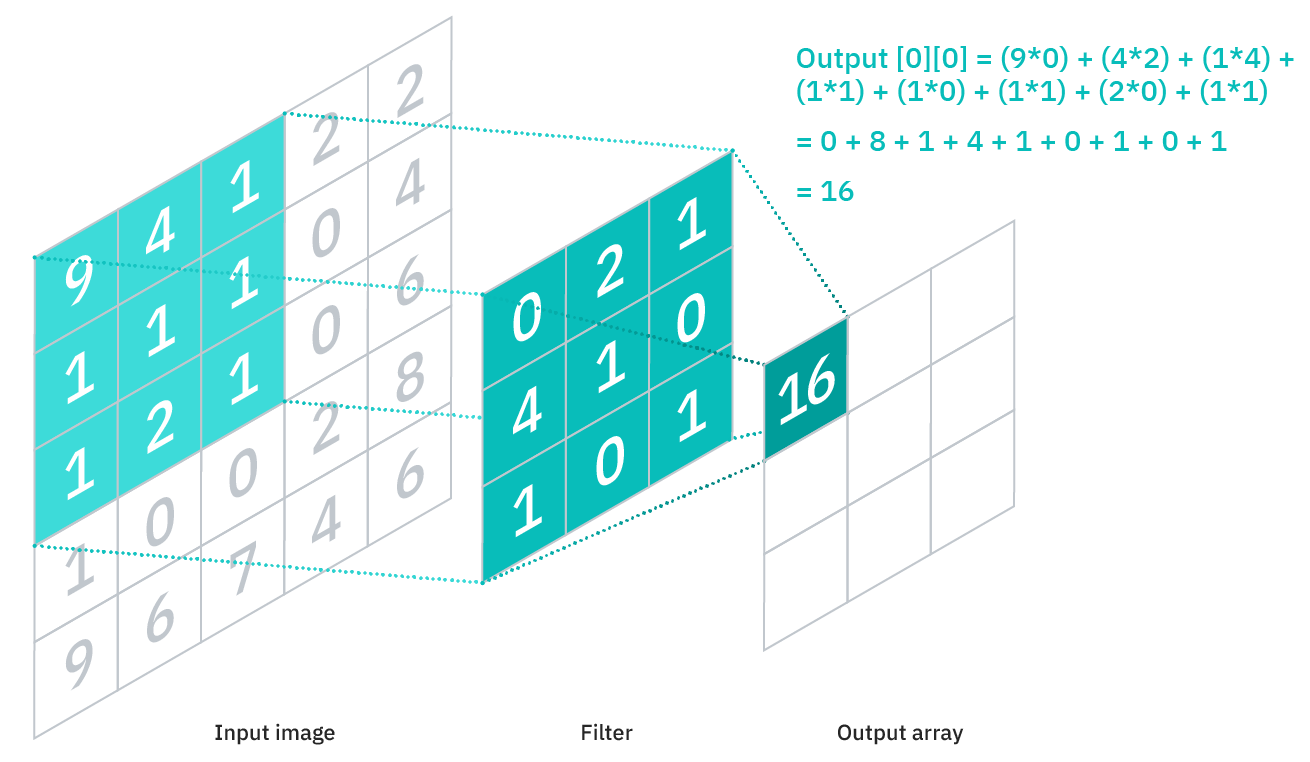
\includegraphics[width=7cm]{./conv1.png}
    \label{conv}
    \caption{Esempio di convolutional layer}
\end{figure}
$\\\\$
È importante citare anche un'altra tipologia di layer sfruttata all'interno del progetto. Questo è chiamato
Global Average Pooling. Lo scopo di tali layer è rimpiazzare i dense layer mediante un'operazione di raggruppamento.
L'idea di base è creare mappe delle caratteristiche per ogni categoria di cui si deve effettuare la 
classificazione. Al posto di aggiungere dei dense layer all'inizio di tale mappa, si esegue una media 
di ogni mappa e il vettore risultante viene passato in un layer softmax in modo da ottenere come risultato 
un tensore di dimensione uno (ossia una sequenza di dati).
\begin{figure}[h]
    \centering
    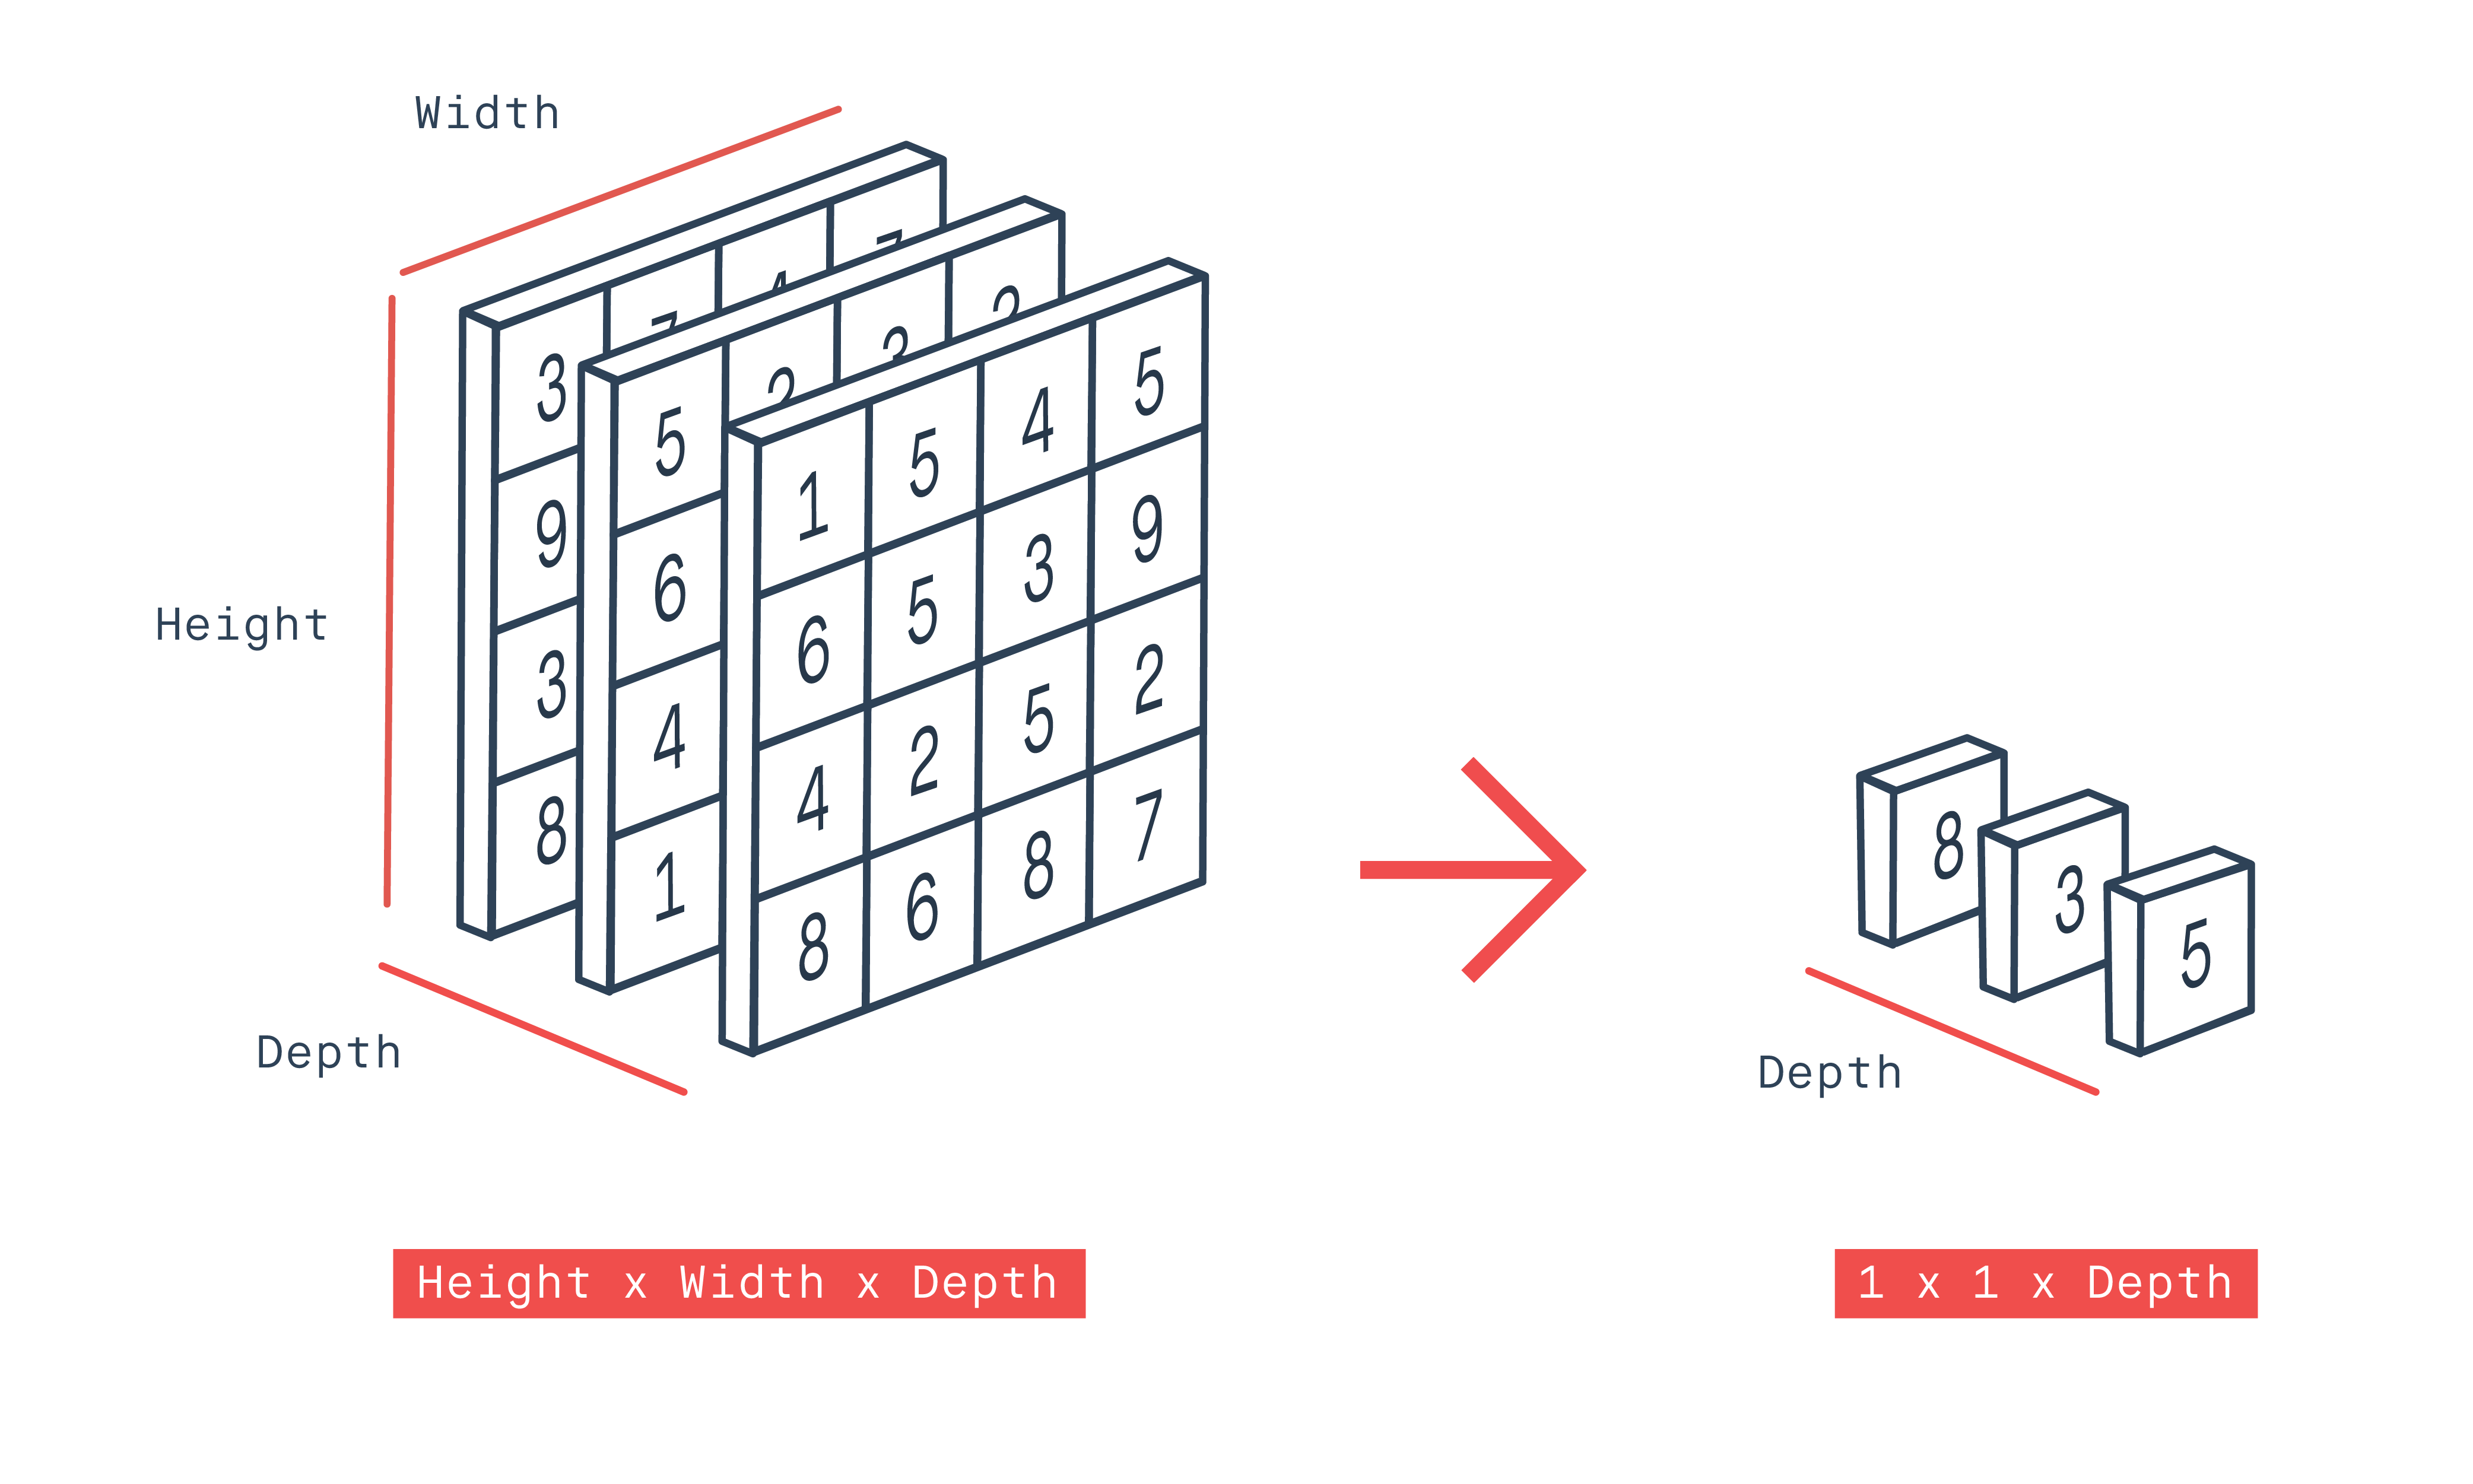
\includegraphics[width=8cm]{./Global_av.png}
    \label{gap}
    \caption{Esempio di Global Average Pooling layer}
\end{figure}
\subsection{Segmentazione delle immagini e U-Net}
\label{Segmentazione delle immagini e U-Net}
Nel caso di classificazione delle immagini la rete neurale assegna un'etichetta (o classe) ad ogni 
immagine in input. Se si vuole conoscere la forma di un oggetto presente nell'immagine, quali pixel appartengono
a quale oggetto o cose simili, si deve assegnare una classe ad ogni pixel dell'immagine e non all'immagine intera.
Tale attività è conosciuta con il nome di segmentazione. 
Grazie a tale tecnica tutti i pixel appartenenti allo stesso oggetto avranno la stesssa etichetta e
sarà più facile compiere analisi più dettagliate sull'immagine.
\\\\
Nel caso del database usato, si è interessati ai soli polmoni del paziente per tale motivo è utile 
effettuare segmentazione in modo da distinguere ciò che fa parte dal polmnone dal resto.
\\\\
Esistono vari modi per effettuare segmentazione delle immagini tra cui:
\begin{itemize}
    \item Segmentazione basata su soglia
    \item Sementazione basata sulle regioni
    \item Segmentazione basata sui margini
    \item Segmentazione basata su gruppi
    \item Segmentazione basata su reti artificiali
\end{itemize}
Nel caso d'interesse si è scelto di usare la segmentazione basata su reti artificiali.
Per tale motivo è stato necessario usare una rete neurale apposita per effettuare segmentazione.
Tale tipologia di rete è conosciuta con il nome di U-Net. Le U-Net sono reti neurali convoluzionali specializzate
nella segmentazioni di immagini biomediche.
\\\\
La U-Net è stata usata per creare delle maschere, ovvero immagini che separano ciò che è all'interno del polmoni 
con ciò che non appartiene ai polmoni. Dunque la previsione che tale rete produce è un'immagine con la 
stessa dimensione dell'immagine iniziale.
\\\\
Dalla maschera creata sarà poi più semplice effettuare ulteriori analisi e modifiche 
sull'immagine iniziale.
\begin{figure}[h]
    \centering
    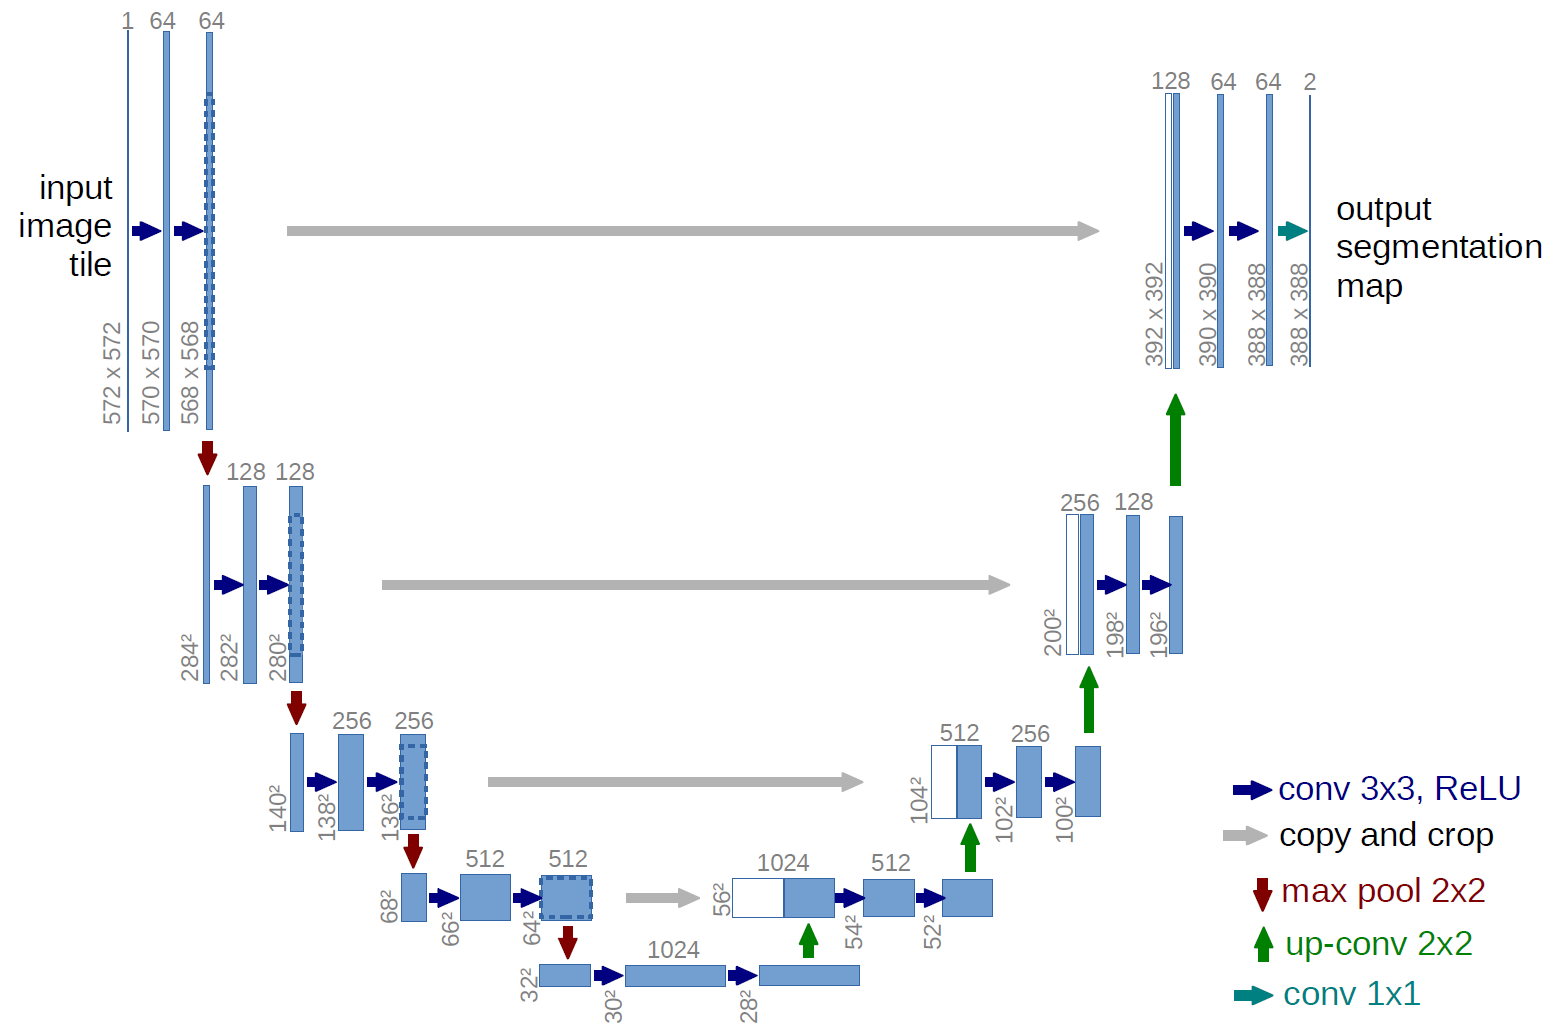
\includegraphics[width=12cm]{./u-net-architecture.png}
    \label{U-Net}
    \caption{Esempio di architettura di una U-Net}
\end{figure}
$\\\\$
$\\\\$
$\\\\$
$\\\\$
\section{Codifica one-hot per dati categorici}
\label{Codifica one-hot per dati categorici}
La codifica one-hot risulta essere molto utile quando si è in presenza di dati categorici. Tale tipologia di dati
contengono etichette relative al dato invece che valori numerici: ogni etichetta solitamente rappresenta 
categorie diverse.
Il problema legato a tale tipologia di dati è che una rete neurale non riesce ad operare direttamente c
sulle etichette dei dati, poiché richiedono che tutte le variabili in ingresso ed uscita siano numeriche.
Per tale motivo si necessita i dati categorici devono essere convertiti in numerici.
La conversione da dati categorici a numerici prevede due passi:
\begin{itemize}
    \item Integer Encoding
    \item One-Hot Encoding
\end{itemize}
Il primo passo prevede che ad ogni categoria venga assegnato un valore numerico, questo potrebbe in 
alcuni casi essere sufficiente per convertire i dati.
Il secondo passo prevede la conversione dei valori numerici in valori binari.
Ciò che solitamente accade è che vengono scelti tanti bit quanti sono le categorie da rappresentare 
e, successivamente, ogni categoria verrà rappresentata da una serie di bit posti come 0 ed un unico bit 
posto ad 1. Di seguito si riporta un esempio di una codifica one-hot sulle categorie utilizzate.
\begin{align*}\label{Esempio di funzione che esegue la codifica one-hot}
    0 \longrightarrow \begin{pmatrix}
        1\\
        0\\
        0
    \end{pmatrix}\\
    1 \longrightarrow \begin{pmatrix}
        0\\
        1\\
        0
    \end{pmatrix}\\
    2 \longrightarrow \begin{pmatrix}
        0\\
        0\\
        1
    \end{pmatrix}
\end{align*}
$\\\\$
Tale processo viene usato all'interno dell'elaborato di tesi al momento dello studio del dataset eterogeneo 
e la realizzazione del multilayer perceptron.
\section{Strumenti usati}
\label{Strumenti usati}
Esistono vari framework per lo sviluppo di reti neurali, uno dei più usati è TensorFlow \cite{tsf}. 
\\
TensorFlow presenta modelli già creati e allenati, i cui pesi possono essere reperiti per effettuare test in manniera rapida.
Insieme all'uso di altre librerie come Keras, l'implementazione di una rete neurale che gestisca i dati a disposizione 
è molto semplificato.
\\
La rete di base usata per partire con l'analisi delle immagini è la MobileNetV2. Tale rete è una CNN che, prendendo come input delle 
immagini.
A tale rete, tuttavia, sono state apportate delle modifiche per via delle dimensioni dell'input e della tipologia di dato 
che si vuole ottenere come previsione.
\\
Oltre a questa tipologia di rete si è sfruttata anche una U-Net, al fine di omogeneizzare tutte le immagini che vengono date come input della MobileNetV2.
La U-Net usata è EfficientNet, con dei pesi preallenati \cite{unw} per riconoscere immagini simili a quelle presenti nel dataset di riferimento.

